\begin{figure}[htbp]
\centering
\begin{tikzpicture}[x=1cm,y=1cm]
\node[anchor=south west,inner sep=0] at (0,0) {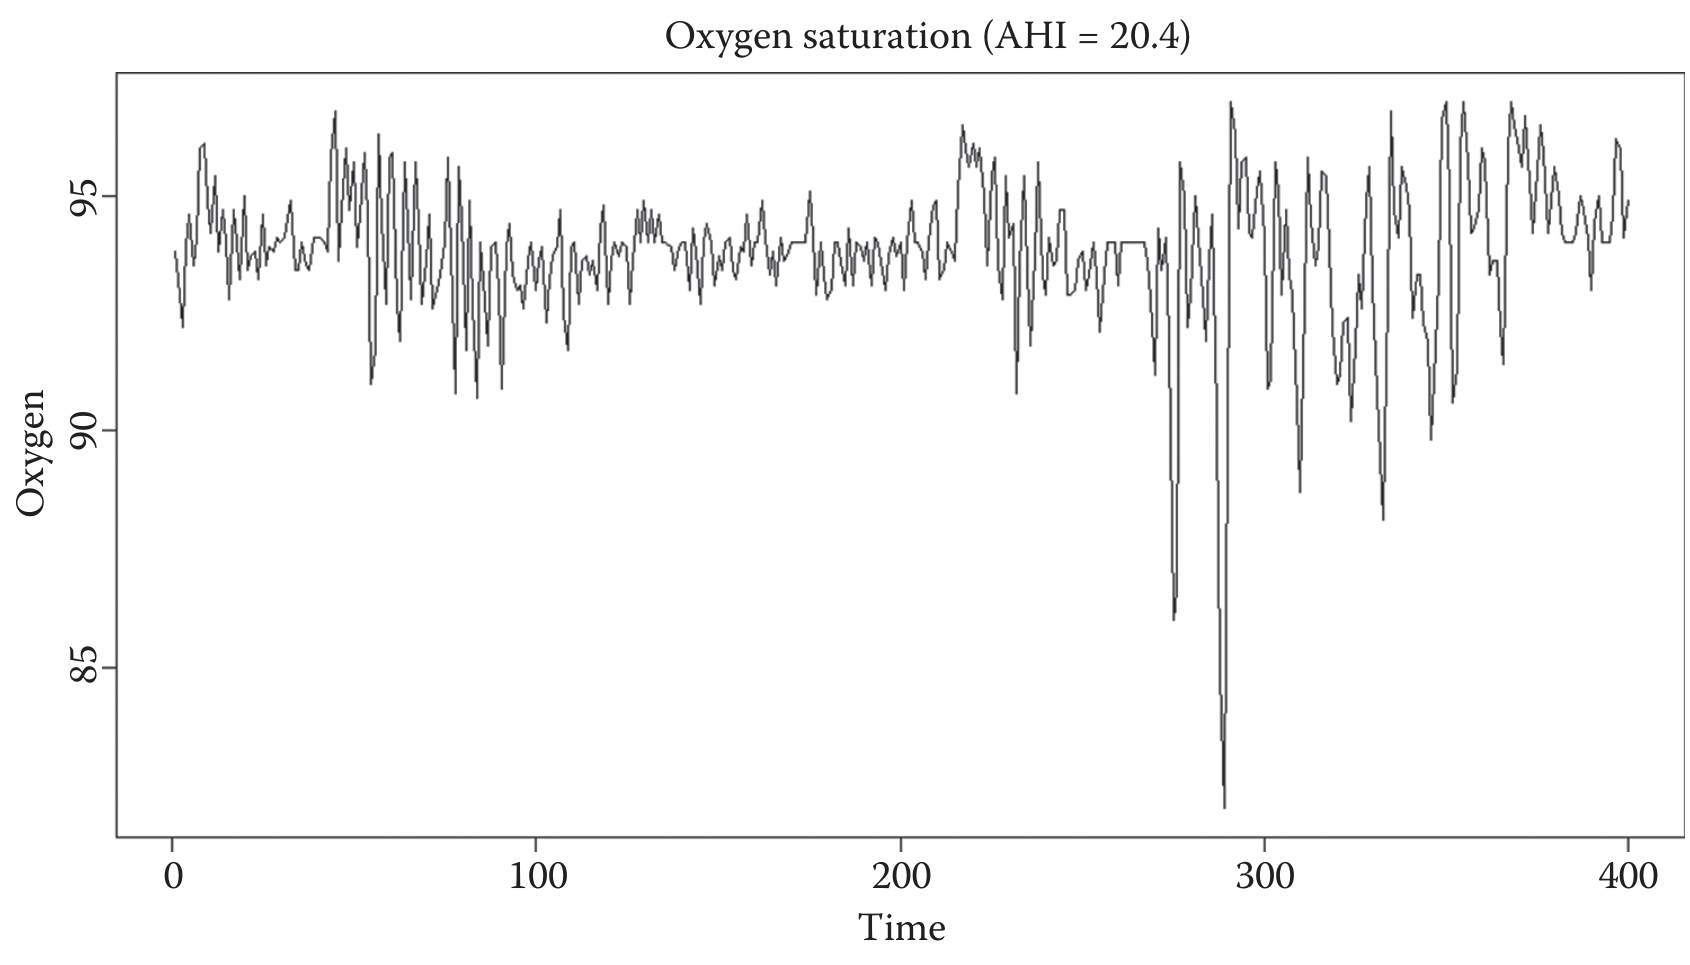
\includegraphics[width=13.8cm]{figures/ch03_fig02_data.png}};
\fill[white] (5.4000,7.3848) rectangle (9.7588,7.7523);
\node[font=\scriptsize,rotate=0,inner sep=0] at (7.5794,7.5686) {血氧饱和度（AHI = 20.4）};
\fill[white] (0.0830,3.6278) rectangle (0.4586,4.7217);
\node[font=\scriptsize,rotate=90,inner sep=0] at (0.2708,4.1747) {血氧};
\fill[white] (6.9743,0.1014) rectangle (7.7523,0.4689);
\node[font=\scriptsize,rotate=0,inner sep=0] at (7.3633,0.2852) {时间};
\end{tikzpicture}
\origfig{2}{血液中的氧浓度。}
\label{fig:ch03-02}
\end{figure}
